\documentclass[11pt,a4paper]{article}

% Document metadata
\title{Example article testing \LaTeX\ features}
\author{Paul D. Bartlett}
\date{2018--2019}

% Make title and author available
\makeatletter
\let\inserttitle\@title
\let\insertauthor\@author
\makeatother

% Packages needed
\usepackage{pgfplots}
\pgfplotsset{compat=1.16}

\usepackage[ps2eps]{abc}

\usepackage{amsmath}
\usepackage{amssymb}
\usepackage{bchart}
\usepackage[style=authoryear-ibid,backend=biber]{biblatex}
\usepackage{booktabs}
\usepackage{chemfig}
\usepackage{chessboard}
\usepackage[basic]{circ}
\usepackage{csvsimple}
\usepackage{cwpuzzle}
\usepackage{dataplot}
\usepackage{fancyhdr}
\usepackage{filecontents}
\usepackage{float}
\usepackage{siunitx}
\usepackage{xskak}

% Put title and author in header
\pagestyle{fancy}
\fancyhf{}
\lhead{``\inserttitle''}
\rhead{\insertauthor}
\addtolength{\headheight}{2pt} % space for the rule

% Add some more unit/prefix definitions
\DeclareSIUnit\bit{b}
\DeclareBinaryPrefix\gibi{Gi}{30}

% Inline datafile
\begin{filecontents*}{data.tmp.csv}
x,y
1,2
3,4
5,6
\end{filecontents*}

% Crossword definition
\begin{filecontents*}{crossword.tmp.tex}
\begin{Puzzle}{3}{3}%
  | [1]B | E | [2]L |.
  |    O | * |    I |.
  | [3]O | N |    E |.
\end{Puzzle}
\begin{PuzzleClues}{\textbf{Across: }}%
  \Clue{1}{BEL}{unit of sound}%
  \Clue{3}{ONE}{Cyrus tooth count}%
\end{PuzzleClues}%
\begin{PuzzleClues}{\textbf{Down: }}%
  \Clue{1}{BOO}{Nickname of \textit{1 across}}%
  \Clue{2}{LIE}{not the truth; or Sweep photo pose}%
\end{PuzzleClues}%
\end{filecontents*}

% Inline bibliography
\begin{filecontents*}{example.tmp.bib}
@book{
  smith2013ex,
  author = "Smith, J.",
  title = "{An Example for Us All}",
  year = 2013,
  publisher = "Practice-Hall Inc."
 }
@book{
  jones2009eg,
  author = "Jones, W.",
  title = "{Examples in Latin}",
  year = 2009,
  publisher = "Cantabridgia Universita Press"
 }
@book{
  foo1999ba,
  author = "Streetcat, R",
  title = "{A Bad Example}",
  year = 1999,
  publisher = "Doesn't Really Matter"
 }
\end{filecontents*}

\addbibresource{example.tmp.bib}

% The document itself
\begin{document}
\maketitle

\begin{abstract}
An example document to showcase and experiment with various \LaTeX\ features that
are useful in different situations---but which would not usually be expected to be used
together in a single document.
\end{abstract}

\tableofcontents
\listoftables
\listoffigures

\section{Equations}

\subsection{Units}
The speed of light, $c$, is \SI{3e8}{\metre\per\second}.\\
Network speeds of \SI[per-mode=symbol]{1}{\gibi\bit\per\second} are now commonplace.

\subsection{Quadratic formula}
\begin{equation}
x = \frac{-b \pm \sqrt{b^2 - 4ac}}{2a}
\end{equation}

\subsection{Maxwell's equations}
\begin{align}
\nabla \cdot \mathbf{D} &= \rho\\
\nabla \cdot \mathbf{B} &= 0\\
\nabla \times \mathbf{E} &= -\frac{\partial \mathbf{B}} {\partial t}\\
\nabla \times \mathbf{H} &= \mathbf{J} + \frac{\partial \mathbf{D}} {\partial t}
\end{align}

\subsection{Inverse of a 2x2 matrix}
\begin{align}
\mathbf{A}^{-1} &= \frac{1}{\det(\mathbf{A})} \operatorname{adj}(\mathbf{A})\\
\begin{pmatrix}
a & b\\
c & d
\end{pmatrix}^{-1}
&=
\frac{1}{ad-bc}
\begin{pmatrix}
d & -b\\
-c & a
\end{pmatrix}
\end{align}

\section{Data handling}

\begin{table}[H]
\centering
\csvautobooktabular{data.tmp.csv}
\caption{Sample data}
\end{table}

\DTLloaddb{data}{data.tmp.csv}
\begin{figure}[H]
\centering
\DTLplot{data}{x=x,y=y,style=lines}
\caption{A line plot}
\end{figure}

\begin{figure}[H]
\centering
\begin{bchart}[step=10,max=50]
\bcbar[text=Yes]{7}
\bcbar[text=No]{42}
\bcbar[text=Maybe]{15}
\bcxlabel{number of responses}
\end{bchart}
\caption{A bar chart}
\end{figure}

\begin{figure}[H]
\centering
\begin{bchart}[plain,max=5]
\bcbar[text=Q1]{2.2}
\bcbar[text=Q2]{-0.6}
\bcbar[text=Q3]{1.1}
\bcxlabel{agreement score}
\end{bchart}
\caption{Another bar chart}
\end{figure}

\begin{figure}[H]
\centering
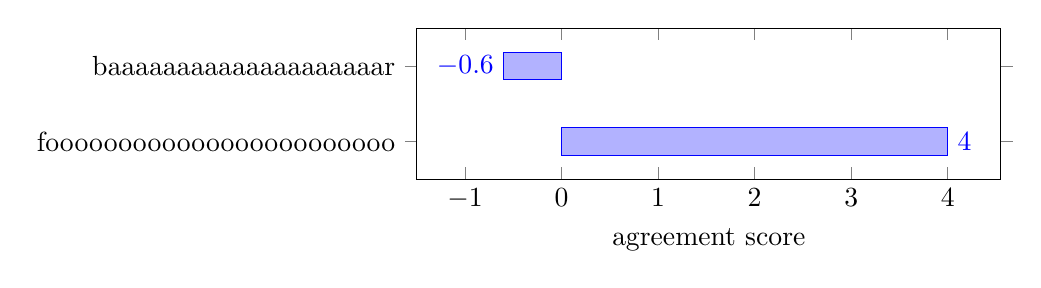
\begin{tikzpicture}
\begin{axis}[
xbar, xmin=-1.5,
width=9cm, height=3.5cm, enlarge y limits=0.5,
xlabel={agreement score},
symbolic y coords={foooooooooooooooooooooooo,baaaaaaaaaaaaaaaaaaaar},
ytick=data,
nodes near coords, nodes near coords align={horizontal},
]
\addplot coordinates {(-0.6,baaaaaaaaaaaaaaaaaaaar) (4,foooooooooooooooooooooooo)};
\end{axis}
\end{tikzpicture}
\caption{Bar chart with \textsc{pgfplots}}
\end{figure}

\section{Chemistry}
\begin{figure}[H]
\centering
\chemfig{H-C(-[2]H)(-[6]H)-C(-[7]O-H)=[1]O}
\caption{Structure of ethanol}
\end{figure}

\section{Electronics}

\begin{figure}[H]
\centering
\begin{circuit}0
\npn1 {?} B l               % transistor
\frompin npn1C              % draw from collector
\- 1 u                      % some wire
\nl\A1 {$I_C$} u            % ammeter for current of collector
\atpin npn1B                % continue drawing from base
\- 1 l                      % some wire
\R1 {510k} l                % resistor
\- 1 l                      % some wire to the edge
\centerto A1                % draw centered to ammeter 1
\nl\A2 {$I_B$} u            % am3emeter 2
\frompin A2b                % link ammeter 2 with resistor
\vtopin R1l
\frompin A1t
\- 1 u
\.1                         % junction
\frompin A2t                % wire to ammeter 2
\vtopin .1
\htopin .1
\- 1 u
\cc\connection1 {$U_b$} c u % driving voltage
\frompin npn1E
\- 1 d
\GND1                       % ground
\end{circuit}
\caption{A simple circuit}
\label{circuit}
\end{figure}

\section{Music}
\begin{figure}[H]
% Set name to Out to match default Out.ps (cannot get options="-O=" to work)
\begin{abc}[program=/Users/pdbartlett/homebrew/bin/abcm2ps,name=Out]
X:4
T:Cronin's Hornpipe
R:hornpipe
S:Keenan and Glackin
E:7
M:C|
L:1/8
K:G
BA|GABc dBde|gage dega|bage dBGB|cABG A2BA|!
GABc dBde|gage dega|bage dBAB|G2G2 G2:|!
fg|afd^c d2ga|bged e2ga|(3bag (3agf gedB|(3cBA AG AcBA|!
GABc dBde|~g3e dega|bage dBAB|G2G2 G2:|!
\end{abc}
\caption{Musical score generated from ABC notation}
\end{figure}

\section{Games \& Puzzles}
\subsection{Chess}
\begin{figure}[H]
\centering
\newchessgame
\hidemoves{1. e4 e5 2. f4}
\chessboard[
  smallboard,
  showmover=false,
  pgfstyle=circle,
  markfield=f4,
]
\caption{King's Gambit}
\end{figure}

\subsection{Crosswords}
\begin{figure}[H]
\input{crossword.tmp.tex}
\caption{Simple crossword}
\end{figure}
\begin{figure}[H]
\PuzzleSolution
\input{crossword.tmp.tex}
\caption{Solution to simple crossword}
\end{figure}

\section{Citations}
Citations can appear in parentheses after text \parencite{smith2013ex}. Or they can be placed
inline as in \textcite{jones2009eg}. There should be two referenced texts in the bibliography
below, as although three were defined one was not cited. Uncited texts can still be shown via
a separate \texttt{refsection} and \texttt{\textbackslash nocite}.

\printbibliography

\begin{refsection}
\nocite{foo1999ba}
\printbibliography[heading=subbibliography, title={Uncited}]
\end{refsection}

\end{document}
